\PassOptionsToPackage{unicode=true}{hyperref} % options for packages loaded elsewhere
\PassOptionsToPackage{hyphens}{url}
%
\documentclass[]{article}
\usepackage{lmodern}
\usepackage{amssymb,amsmath}
\usepackage{ifxetex,ifluatex}
\usepackage{fixltx2e} % provides \textsubscript
\ifnum 0\ifxetex 1\fi\ifluatex 1\fi=0 % if pdftex
  \usepackage[T1]{fontenc}
  \usepackage[utf8]{inputenc}
  \usepackage{textcomp} % provides euro and other symbols
\else % if luatex or xelatex
  \usepackage{unicode-math}
  \defaultfontfeatures{Ligatures=TeX,Scale=MatchLowercase}
\fi
% use upquote if available, for straight quotes in verbatim environments
\IfFileExists{upquote.sty}{\usepackage{upquote}}{}
% use microtype if available
\IfFileExists{microtype.sty}{%
\usepackage[]{microtype}
\UseMicrotypeSet[protrusion]{basicmath} % disable protrusion for tt fonts
}{}
\IfFileExists{parskip.sty}{%
\usepackage{parskip}
}{% else
\setlength{\parindent}{0pt}
\setlength{\parskip}{6pt plus 2pt minus 1pt}
}
\usepackage{hyperref}
\hypersetup{
            pdfborder={0 0 0},
            breaklinks=true}
\urlstyle{same}  % don't use monospace font for urls
\usepackage[margin=1in]{geometry}
\usepackage{longtable,booktabs}
% Fix footnotes in tables (requires footnote package)
\IfFileExists{footnote.sty}{\usepackage{footnote}\makesavenoteenv{longtable}}{}
\usepackage{graphicx,grffile}
\makeatletter
\def\maxwidth{\ifdim\Gin@nat@width>\linewidth\linewidth\else\Gin@nat@width\fi}
\def\maxheight{\ifdim\Gin@nat@height>\textheight\textheight\else\Gin@nat@height\fi}
\makeatother
% Scale images if necessary, so that they will not overflow the page
% margins by default, and it is still possible to overwrite the defaults
% using explicit options in \includegraphics[width, height, ...]{}
\setkeys{Gin}{width=\maxwidth,height=\maxheight,keepaspectratio}
\setlength{\emergencystretch}{3em}  % prevent overfull lines
\providecommand{\tightlist}{%
  \setlength{\itemsep}{0pt}\setlength{\parskip}{0pt}}
\setcounter{secnumdepth}{0}
% Redefines (sub)paragraphs to behave more like sections
\ifx\paragraph\undefined\else
\let\oldparagraph\paragraph
\renewcommand{\paragraph}[1]{\oldparagraph{#1}\mbox{}}
\fi
\ifx\subparagraph\undefined\else
\let\oldsubparagraph\subparagraph
\renewcommand{\subparagraph}[1]{\oldsubparagraph{#1}\mbox{}}
\fi

% set default figure placement to htbp
\makeatletter
\def\fps@figure{htbp}
\makeatother

\usepackage{xcolor}

\author{}
\date{\vspace{-2.5em}}

\begin{document}

{
\setcounter{tocdepth}{2}
\tableofcontents
}
\hypertarget{a-comparison-across-clinics-and-between-pilgrim-and-peripheral-sites}{%
\subsection{A comparison across clinics and between pilgrim and
peripheral
sites}\label{a-comparison-across-clinics-and-between-pilgrim-and-peripheral-sites}}

\begin{center}\rule{0.5\linewidth}{0.5pt}\end{center}

The aim of this project is to audit our use of general surgery and
colorectal surgery clinics. We acquired our clinic attendance data from
hospital information services. We further analysed this data to assess
our utilization and DNAs. These are the clinic codes use for the purpose
of this analysis \textbf{JH-MIRO2, JH-ZAIO4, PH-ATE35, PH-ATEPF,
PH-GOR52, PH-MIR41, PH-MIRPF, PH-MMC35, PH-MOB21, PH-MOB40, PH-RTH11,
PH-RTH45, PH-ZAI50, SD-MMCSD, SD-ATESD}

\begin{center}\rule{0.5\linewidth}{0.5pt}\end{center}

\hypertarget{the-data}{%
\subsection{1.The Data}\label{the-data}}

With a preliminary view we can see that our \textcolor{blue}{Pilgrim
Median Booking Rate}:91.7\% is marginally higher than our
\textcolor{red}{Peripheral Median Booking Rate}:89.5\%. Difference in
median was found to be statistically significant at p-value of
\emph{0.023}(Graph 1.1A). Similarly our \textcolor{blue}{Pilgrim Median
Utilizaton Rate}:83.3\% is marginally higher than our
\textcolor{red}{Peripheral Median Utilization Rate}:79.2\%. Difference
in median was found to be statistically significant at p-value of
\emph{0.011}(Graph 1.1B)

\hypertarget{graph-1.1}{%
\subsubsection{Graph 1.1}\label{graph-1.1}}

\begin{center}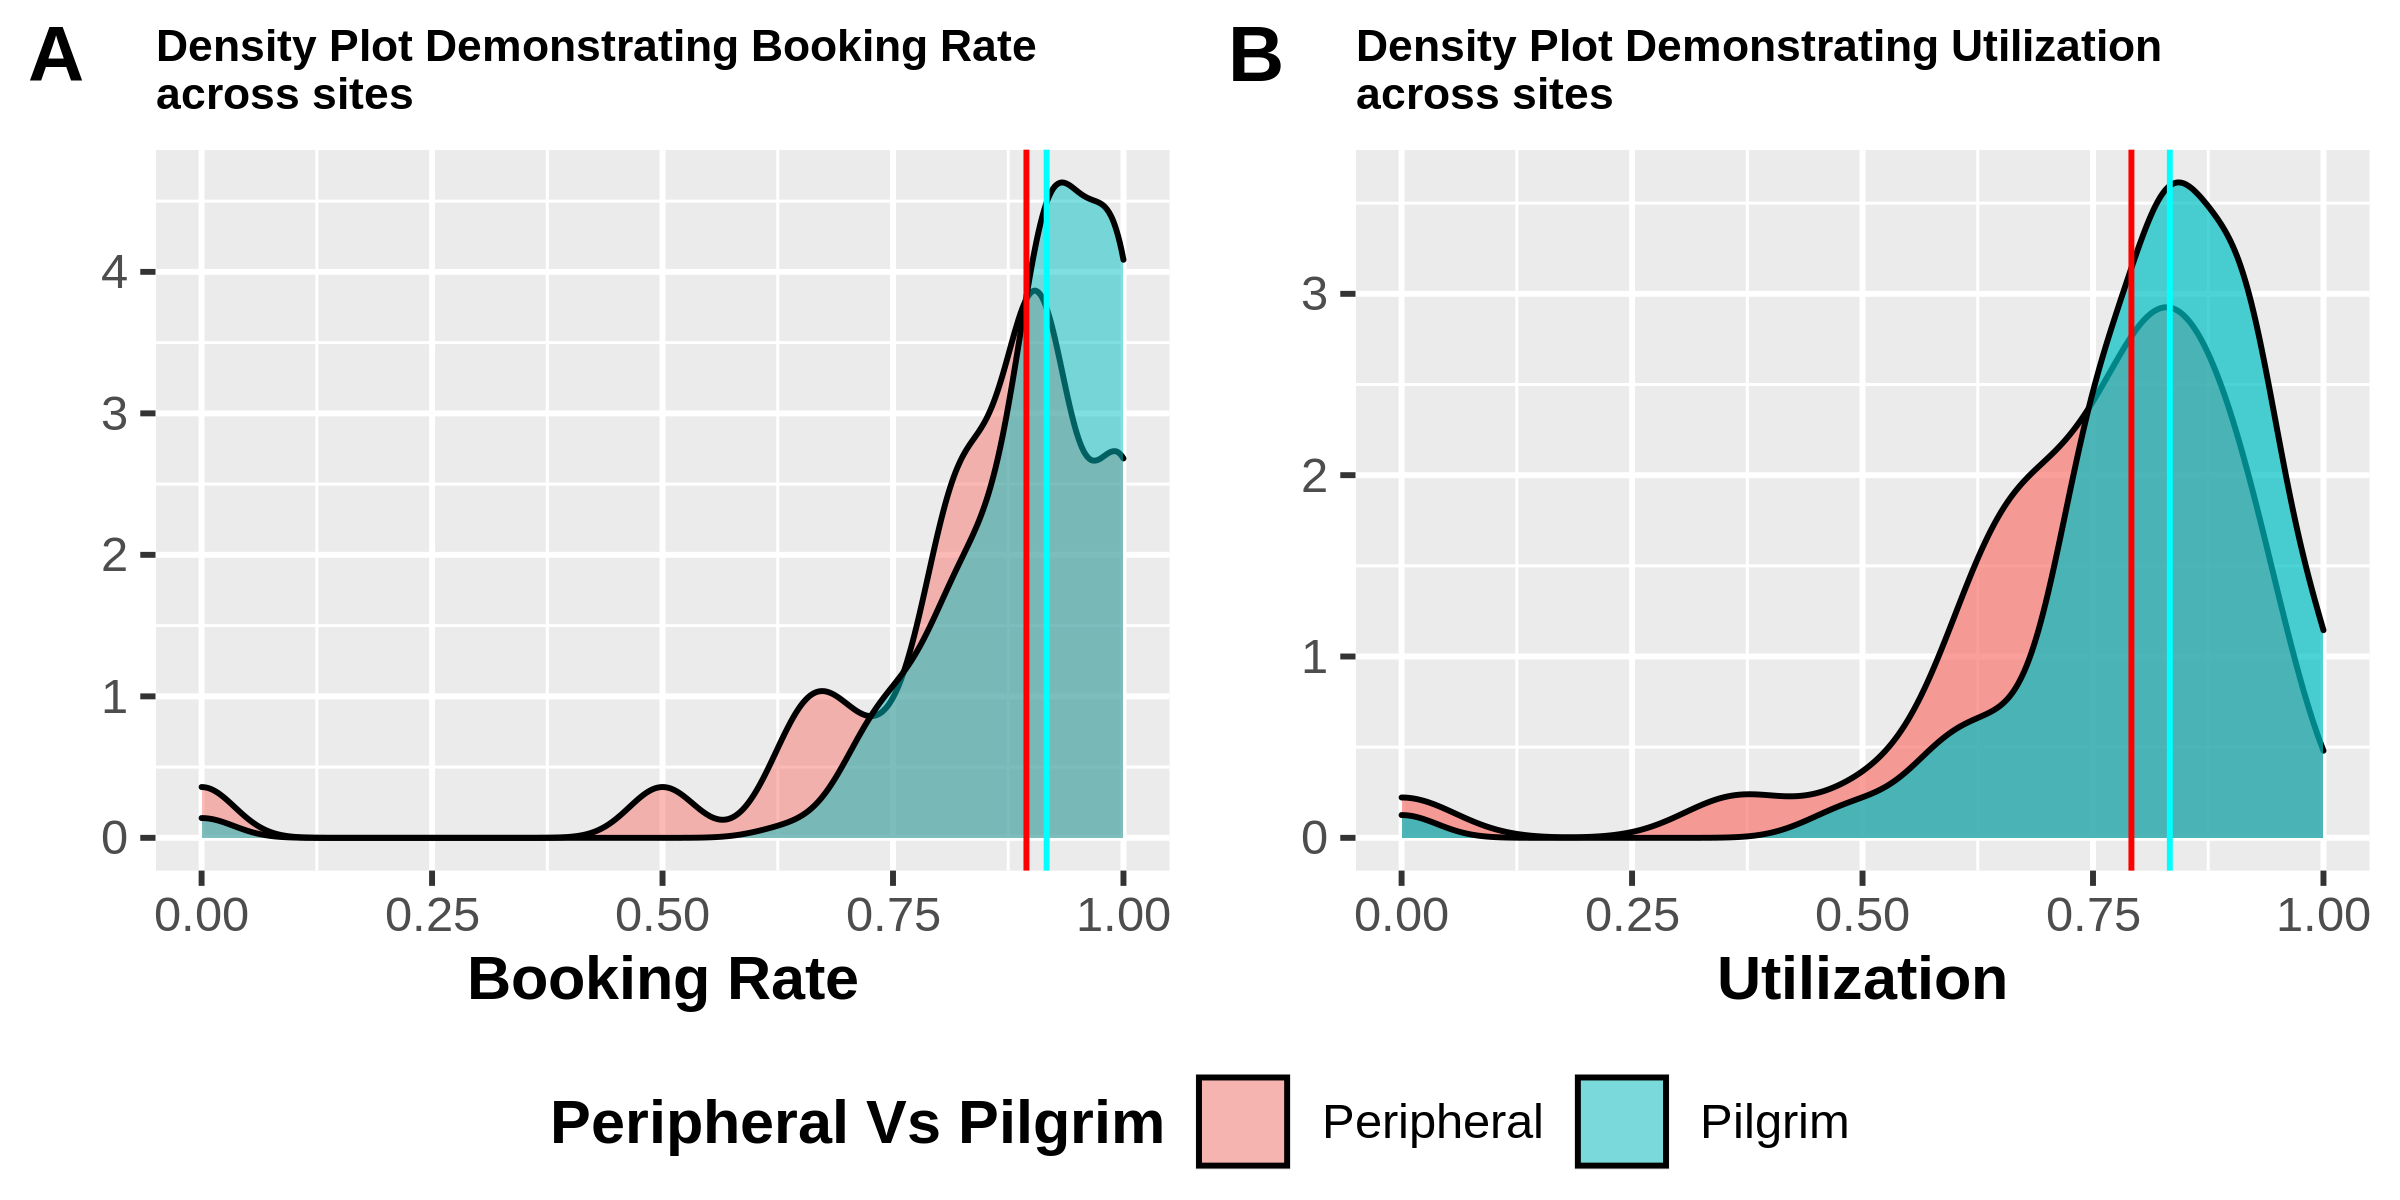
\includegraphics{LF2_files/figure-latex/unnamed-chunk-3-1} \end{center}

\hypertarget{table-1-total-number-of-one-and-two-man-clinics-per-month-for-pilgrim-and-peripheral-sites}{%
\subsubsection{Table 1: Total number of One and Two Man Clinics Per
Month for Pilgrim and Peripheral
Sites}\label{table-1-total-number-of-one-and-two-man-clinics-per-month-for-pilgrim-and-peripheral-sites}}

\begin{table}

\centering
\begin{tabular}[t]{llrl}
\toprule
M & OneVsTwo & count & Site\\
\midrule
Aug & One Man & 2 & Peripheral\\
Aug & One Man & 13 & Pilgrim\\
Sep & One Man & 1 & Peripheral\\
Sep & One Man & 13 & Pilgrim\\
Oct & One Man & 3 & Peripheral\\
\addlinespace
Oct & One Man & 17 & Pilgrim\\
Nov & One Man & 6 & Peripheral\\
Nov & One Man & 20 & Pilgrim\\
Dec & One Man & 5 & Peripheral\\
Dec & One Man & 13 & Pilgrim\\
\addlinespace
Jan & One Man & 2 & Peripheral\\
Jan & One Man & 18 & Pilgrim\\
\bottomrule
\end{tabular}
\centering
\begin{tabular}[t]{llrl}
\toprule
M & OneVsTwo & count & Site\\
\midrule
Aug & Two Man & 2 & Peripheral\\
Aug & Two Man & 14 & Pilgrim\\
Sep & Two Man & 4 & Peripheral\\
Sep & Two Man & 9 & Pilgrim\\
Oct & Two Man & 2 & Peripheral\\
\addlinespace
Oct & Two Man & 17 & Pilgrim\\
Nov & Two Man & 10 & Pilgrim\\
Dec & Two Man & 2 & Peripheral\\
Dec & Two Man & 10 & Pilgrim\\
Jan & Two Man & 2 & Peripheral\\
\addlinespace
Jan & Two Man & 11 & Pilgrim\\
\bottomrule
\end{tabular}
\end{table}

\hypertarget{graph-1.2-histogram-demonstrating-the-distribution-of-clinic-utilizatation-rates}{%
\subsubsection{Graph 1.2 Histogram demonstrating the distribution of
Clinic Utilizatation
Rates}\label{graph-1.2-histogram-demonstrating-the-distribution-of-clinic-utilizatation-rates}}

\begin{center}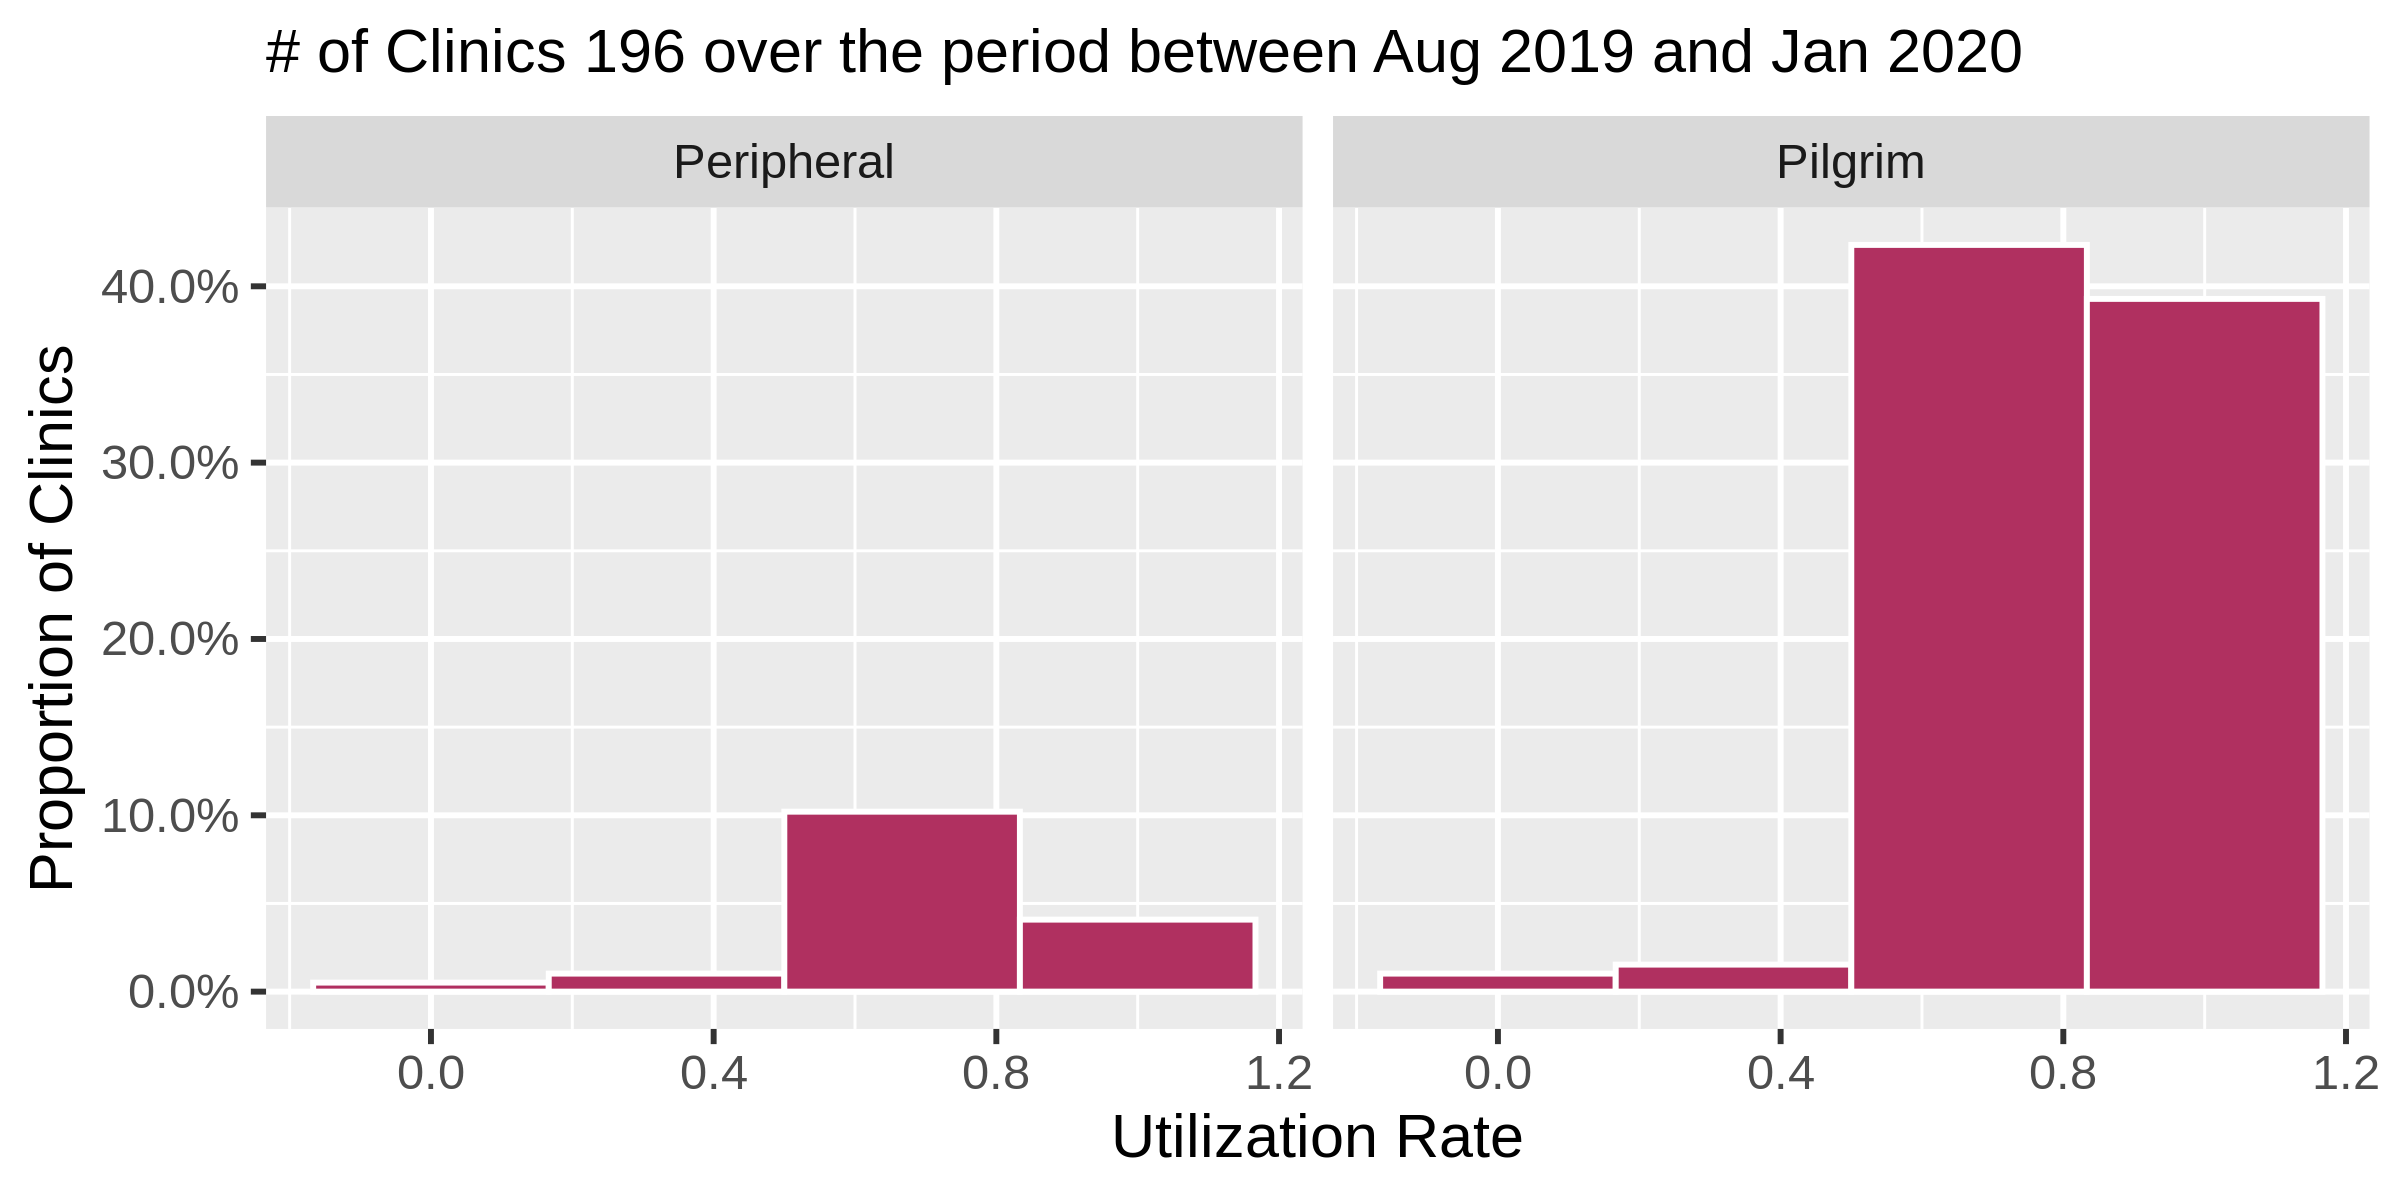
\includegraphics{LF2_files/figure-latex/unnamed-chunk-5-1} \end{center}

\hypertarget{further-breakdown}{%
\subsection{2.Further Breakdown}\label{further-breakdown}}

The following graphs demonstrate per clinic data.
\textcolor{black}{\textbf{Black Shapes}} demonstrate booking rate while
\textcolor{red}{\textbf{Red Shapes}} demonstrate utilization rates.
These are monthly rates ie the actual figure is an average of clinics
used per month. \textbf{Booking rate} is
\[\frac{initial\ booked slots}{total\ available\ slots}\] while
\textcolor{red}{\textbf{Utilization Rate}} is
\[\frac{attended \ clinic\  slots}{booked\ slots}\]

\hypertarget{graph-2.1-booking-and-utilization-rate-per-month-for-one-man-clinics}{%
\subsubsection{Graph 2.1 Booking and Utilization rate per month for One
Man
clinics}\label{graph-2.1-booking-and-utilization-rate-per-month-for-one-man-clinics}}

\begin{center}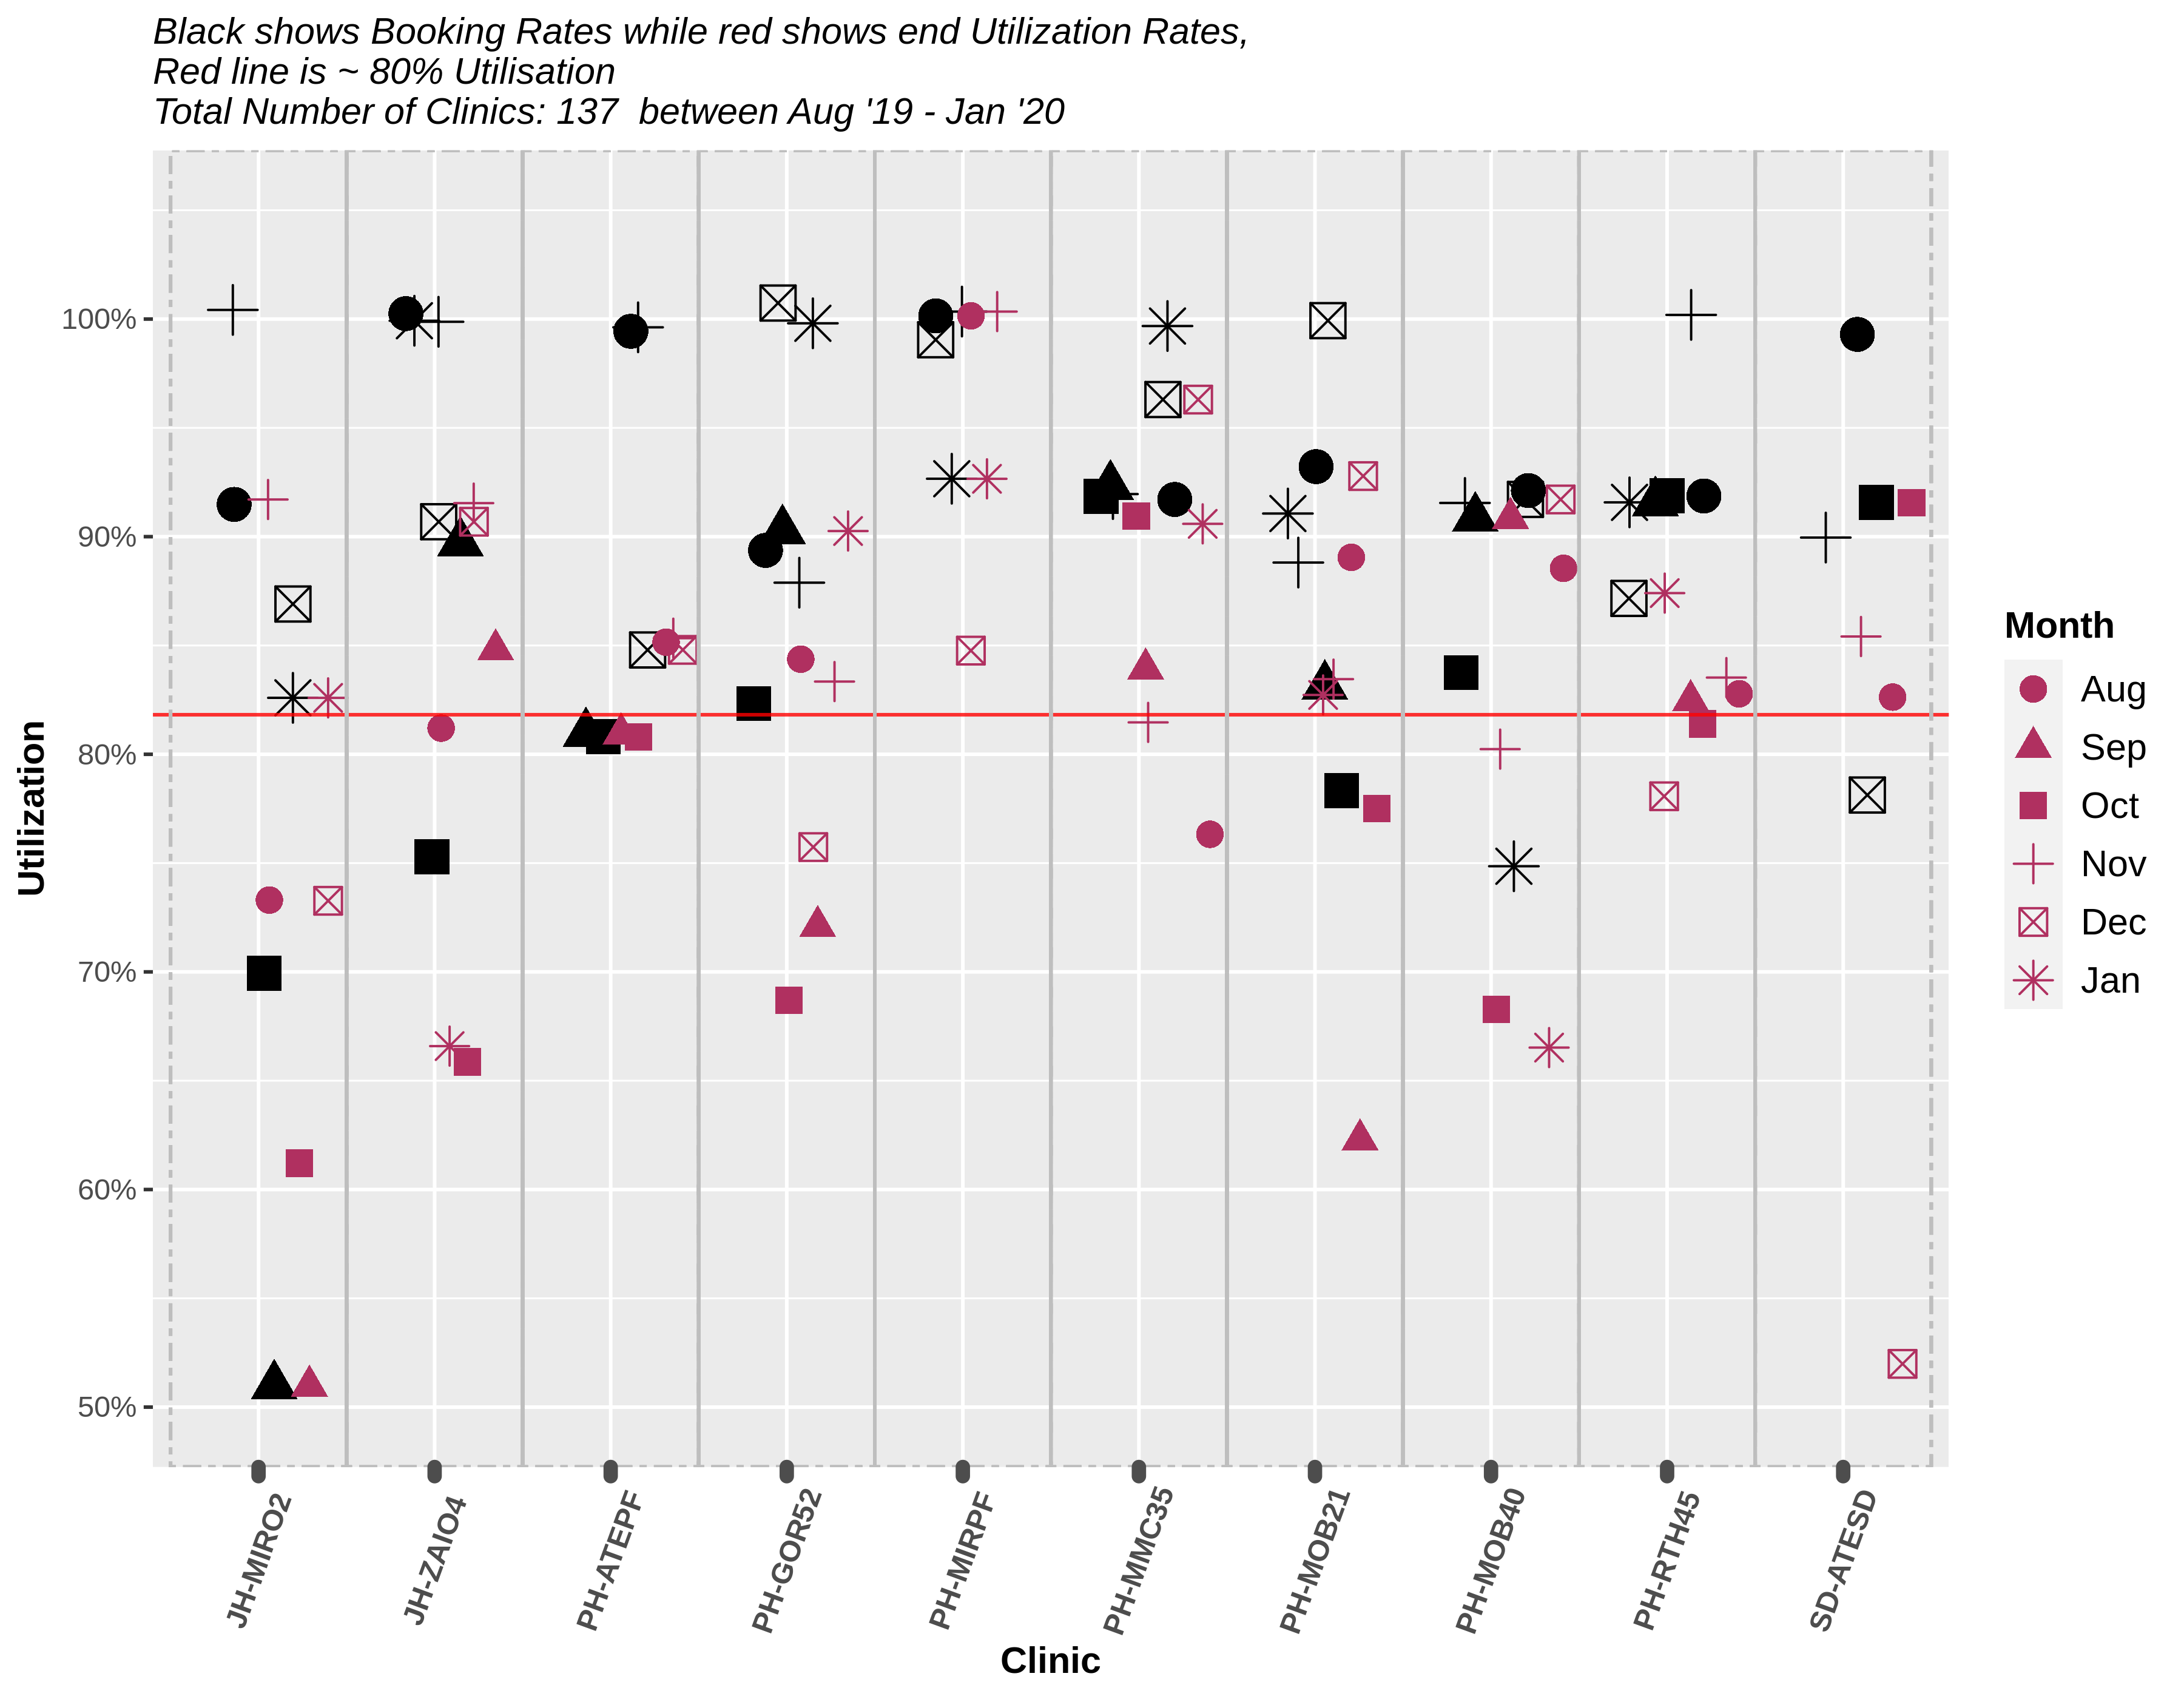
\includegraphics{LF2_files/figure-latex/unnamed-chunk-6-1} \end{center}

\hypertarget{graph-2.2-booking-and-utilization-rates-per-month-for-two-man-clinics}{%
\subsubsection{Graph 2.2 Booking and Utilization Rates per month for Two
Man
clinics}\label{graph-2.2-booking-and-utilization-rates-per-month-for-two-man-clinics}}

\begin{center}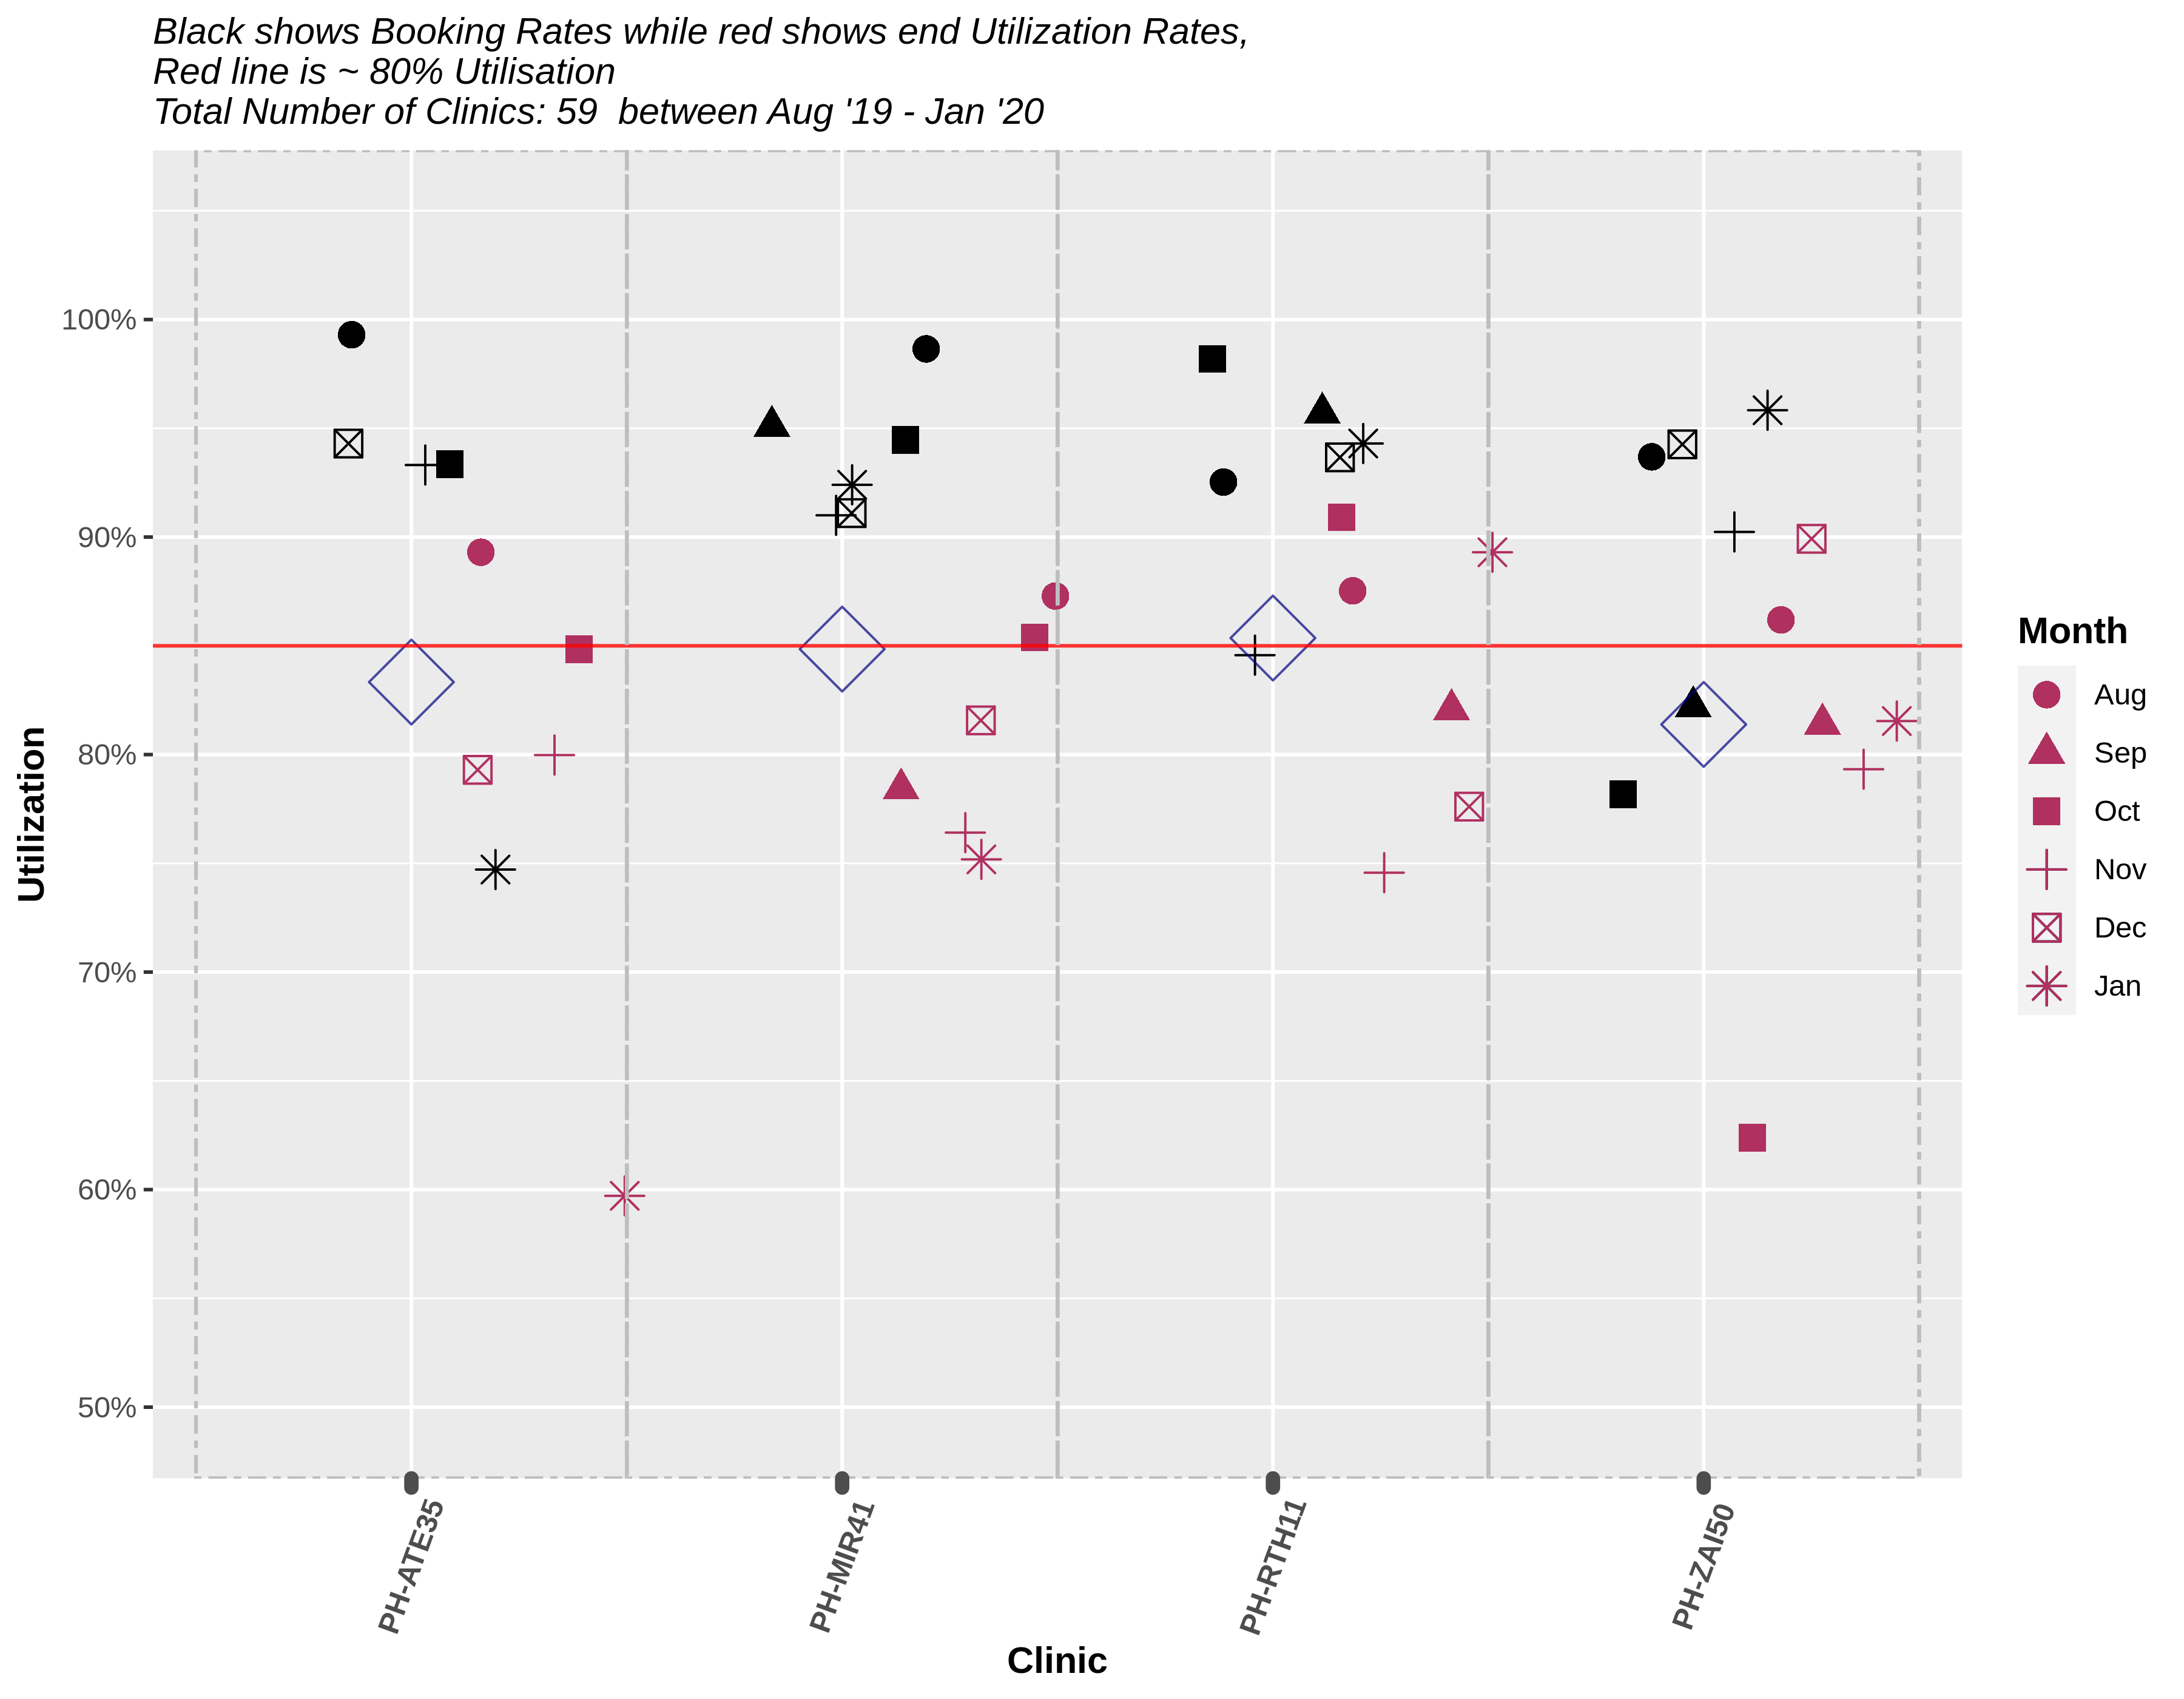
\includegraphics{LF2_files/figure-latex/unnamed-chunk-7-1} \end{center}

\hypertarget{graph-2.3-utilization-and-booking-rate-per-month-across-peripheral-vs-pilgrim-clinics}{%
\subsubsection{Graph 2.3 Utilization and Booking Rate per month across
Peripheral vs Pilgrim
clinics}\label{graph-2.3-utilization-and-booking-rate-per-month-across-peripheral-vs-pilgrim-clinics}}

\begin{center}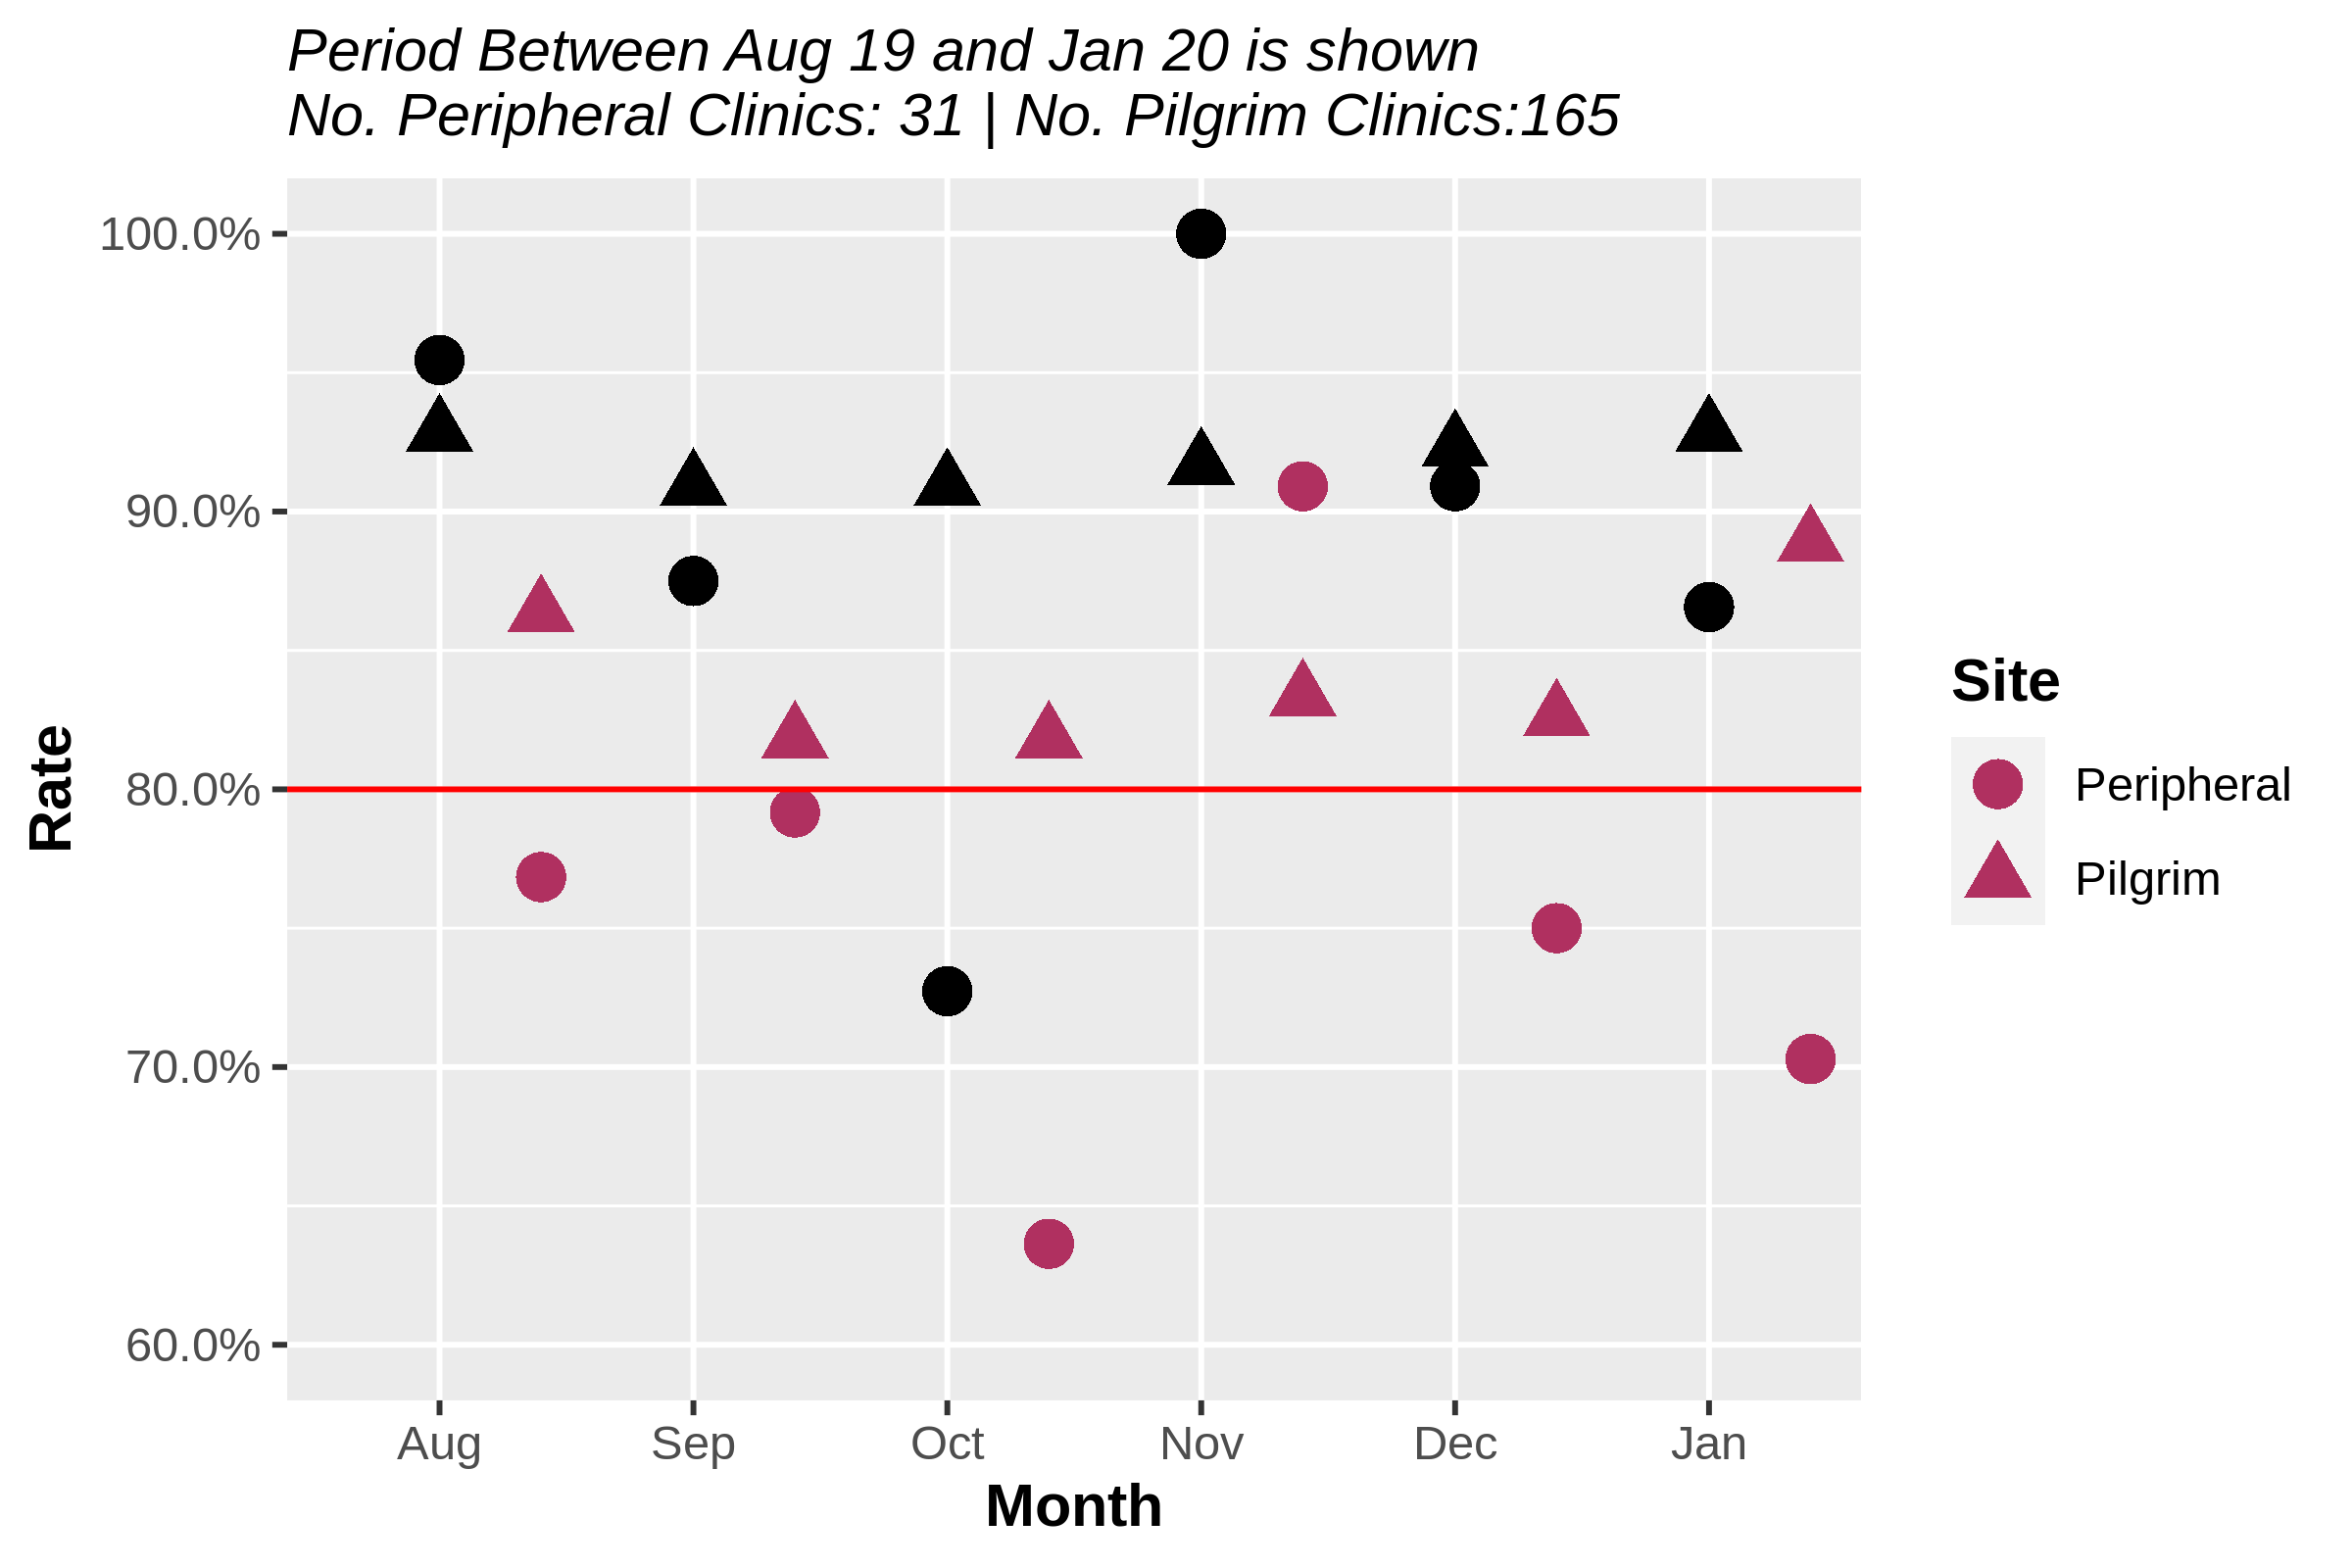
\includegraphics{LF2_files/figure-latex/unnamed-chunk-8-1} \end{center}

\hypertarget{graph-2.4-utilization-and-booking-rate-per-month-across-peripheral-vs-pilgrim-clinics}{%
\subsubsection{Graph 2.4 Utilization and Booking Rate per month across
Peripheral vs Pilgrim
clinics}\label{graph-2.4-utilization-and-booking-rate-per-month-across-peripheral-vs-pilgrim-clinics}}

\begin{center}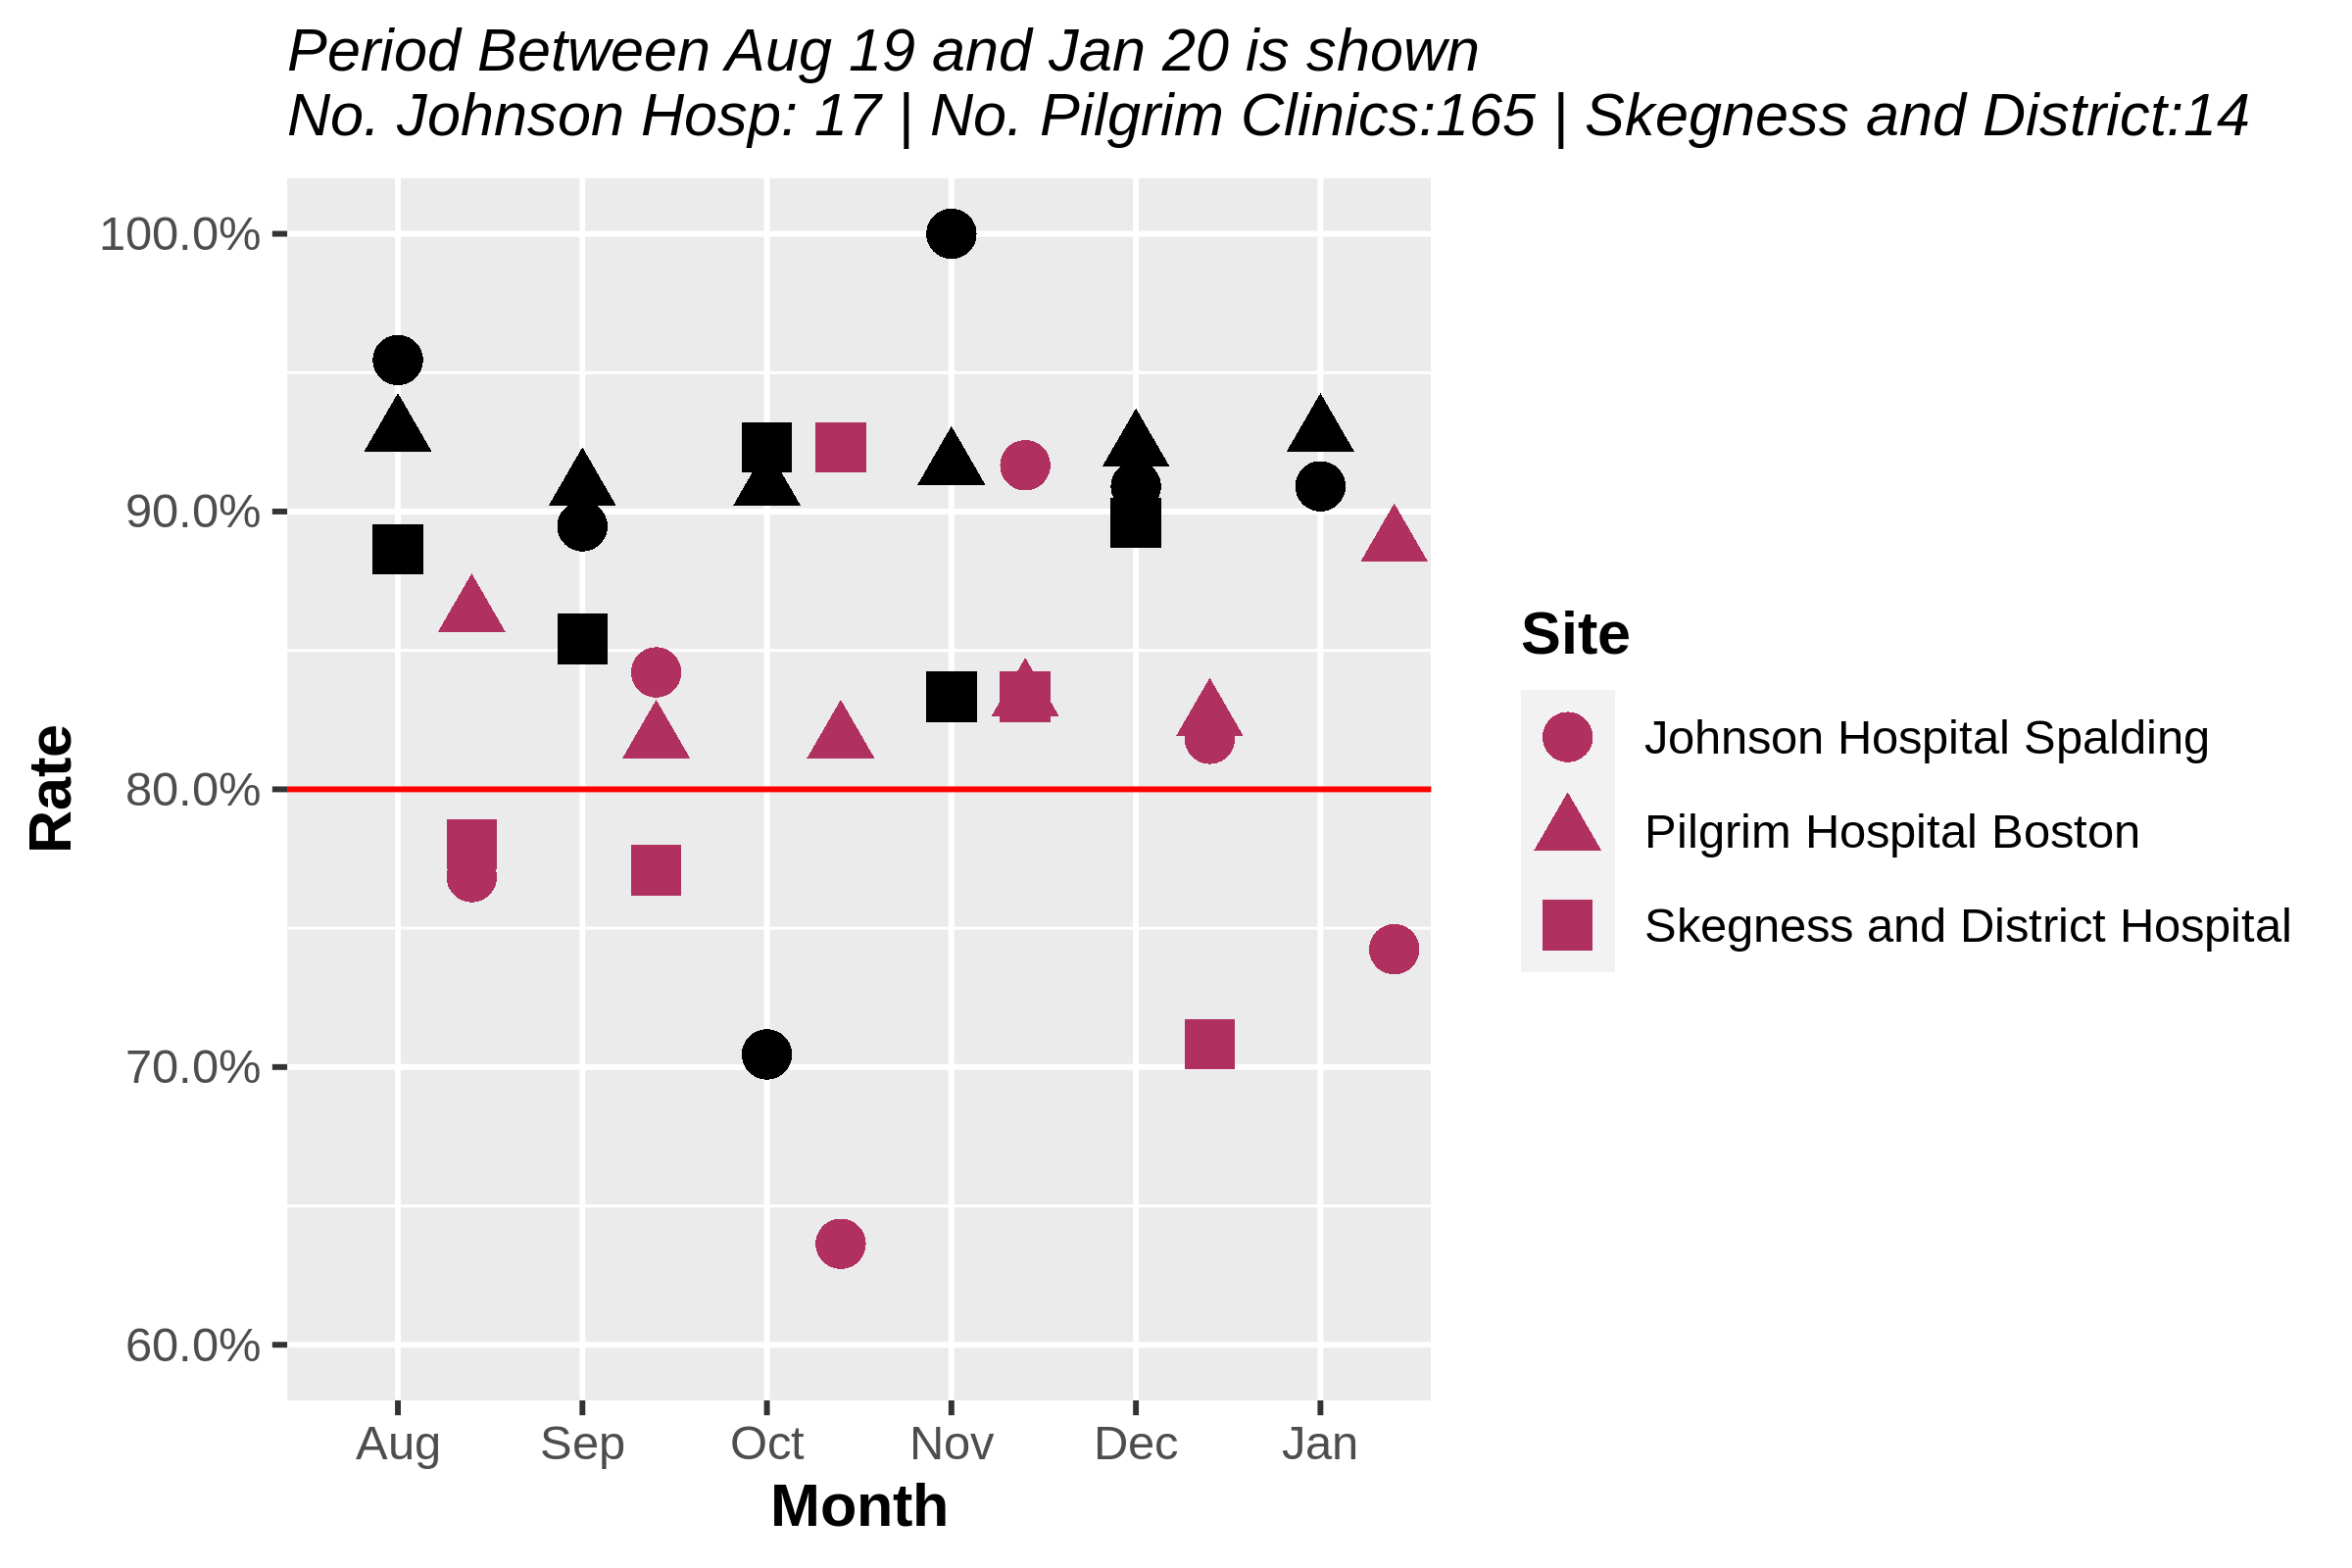
\includegraphics{LF2_files/figure-latex/unnamed-chunk-9-1} \end{center}

\begin{center}\rule{0.5\linewidth}{0.5pt}\end{center}

\hypertarget{discussion}{%
\subsection{3.Discussion}\label{discussion}}

\protect\hyperlink{graph-2.4}{Graph 2.4} \&
\protect\hyperlink{graph-2.3}{Graph 2.3} demonstrates again
underutilized peripheral clinics clinics(p-value:0.011) despite having
similar Booking Rates. This appears to be more during certain month.
Again however due the small sample sizes it is not possible to perform
adequate analysis.

Initially it seems that the differences although statistically
significant were small. However when consulting the last 4 charts it
seems evident that a notable number of our clinics were underbooked at
80\% booking rate(which translates to 2 clinic slots for 1-man-clinics
and about 3 clinic slots for 2-man-clinics). Although those numbers
warrant attention their statistical significance is not easily
demonstrated due to the small sample sizes(As shown on table 1). If we
were to assume their significance the next question we need to answer is
\emph{why?}.

\begin{itemize}
\tightlist
\item
  Why are our \textbf{Booking rates} occasionally/frequently falling
  below our arbitrary 80\%?
\item
  Why are we having low \textcolor{red}{\textbf{Utilization Rate}}? Is
  it something we need to capitalize on?
\end{itemize}

And Finally the next pertinent question is do we that small of a
population to explain our underutilization?\\
***

\hypertarget{recommendations}{%
\subsection{4.Recommendations}\label{recommendations}}

\end{document}
